\chapter{Cluster Analysys}
\label{ch:cluster}

\section{Introduzione alla Cluster Analysys}

    Lorem ecc

\section{Algoritmi di Clustering}

    \subsection{Algoritmo K-Means di Weka}
        Lorem ecc

        \begin{figure}
            \centering
            \caption{finestra che mostra i parametri impostabili dell'algoritmo K-Means}
            \label{kmeans_weka}
            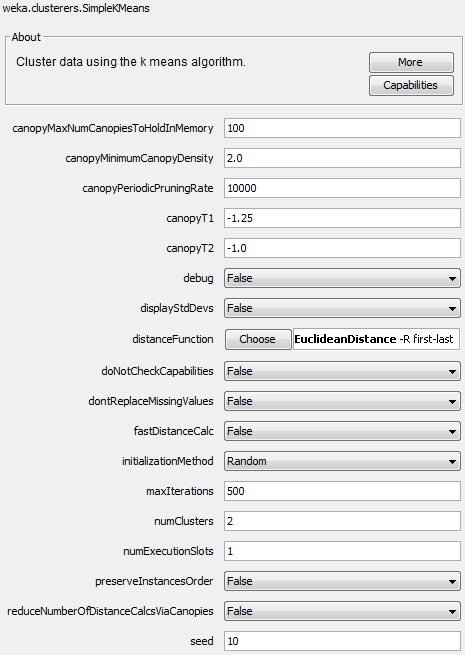
\includegraphics[scale=0.50]{img/cluster_k_means.png}
        \end{figure}

    \subsection{Algoritmo DBSCAN di Weka}
        Lorem ecc

        \begin{figure}
            \centering
            \caption{finestra che mostra i parametri impostabili dell'algoritmo DBSCAN}
            \label{dbscan_weka}
            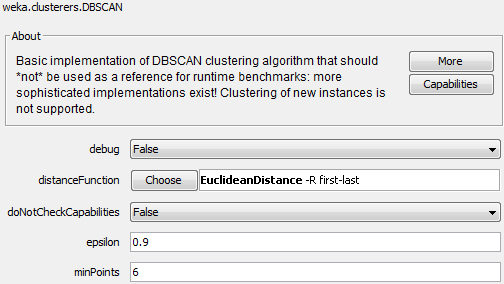
\includegraphics[scale=0.50]{img/dbscan_weka.png}
        \end{figure}

    \subsection{Algoritmo di Clustering Gerarchico}

        \begin{figure}
            \centering
            \caption{finestra che mostra i parametri impostabili dell'algoritmo di clustering gerarchico}
            \label{hierar_weka}
            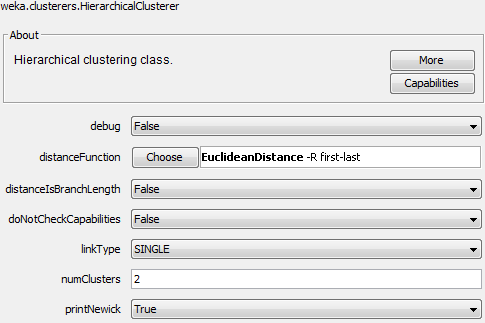
\includegraphics[scale=0.50]{img/hierarch_weka.png}
        \end{figure}

\section{Clustering sulle Valutazioni dei Corsi}

    \subsection{Lancio di K-Means e analisi dei risultati}

    \subsection{Tentativo di utilizzo di DBSCAN}

\section{Clustering sulla Produttività degli Studenti}

    ...

    \subsection{Clustering Gerarchico}

\section{Clustering sulla join dei due data set}

    \subsection{Lancio di $K-Means$}

    \subsection{Analisi dei risultati di $K-Means$}